\section{Literaturrecherche}

\subsection{Allgemeines Vorgehen}

Es wurden folgende Schritte unternommen um einen möglichst umfangreichen Überblick über alle verfügbaren Quellen zu erhalten:
\begin{enumerate}
\item TODO
\item TODO
\end{enumerate}
In Tabelle [TODO REF] ist eine Übersicht über alle genutzen Ressourcen zu finden. Ab Seite \pageref{startdetails} werden die Ergebnisse und Erfahrungen mit diesen Ressourcen näher vorgestellt.

%TODO Links auf die ganzen Seiten in der Tabelle
%TODO anti blocksatz in ressource und tabelle breiter
\renewcommand{\arraystretch}{1.5}
\begin{longtable}{p{3.6cm}|p{3.5cm}|l|p{3.5cm}}
Resourcentyp & Resource & Datum & Suchergebnisse\\\hline\endhead
\endfoot\endlastfoot
Literaturdatenbank/ Bibliothek & DHBW Bibliothek & 26.02.2013 & 5 nutzbare Ergebnisse\\
Offizielle Dokumentation & Oracle & 28.02.2013 & verschiedene (siehe Abschnitt \ref{oracle})\\
Patentdatenbank & Deutsches Patent- und Markenamt & 26.02.2013 & 2476x Java (Titel), 0x Java 7 (Titel), 3521x Java 7 (Volltext), keine nutzbaren Ergebnisse\\
Literaturdatenbank & Association for Computing Machinery & 27.02.2013 & 45637 Treffer, davon 1 vielversprechend.\\
Literaturdatenbank & Search Data Backup & 27.02.2013 & viele Relevante Treffer, davon 6 ausgewählt.\\
Digital Library & IEEE xplore & 27.02.2012 & keine nutzbaren Dokumente\\
Literaturdatenbank & FIZ Technik/ WFi Frankfurt & 27.02.2012 & keine nutzbaren Dokumente\\
Literaturdatenbank/ Bibliothek & Milibib/ Oldenbourg Akademie Link & 27.02.2013 & 57 Ergebnisse, 1 Titel Ausgewählt\\
Internetquelle & Google & 27.02.2013 & sehr viele Treffer, davon 5 ausgewählt (teilweise Duplikate zu anderen Quellen)\\
Internetquelle & Wikipedia & 27.02.2013 & 5 Treffer (über Google gesucht)\\
Literaturdatenbank & Elektronische Zeitschriftenbibliothek & 27.02.2013 & keine relevanten Ergebnisse\\
Literaturdatenbank & SpringerLink & 27.02.2013 & mehr als 100.000 Treffer, davon 1 vielversprechend\\
Literaturdatenbank & Books24x7 & 27.02.2013 & 2302 Treffer, 1 sehr relevant\\
Videodatenbank & Video2Brain & 27.02.2013 & 17 Treffer, 1 sehr relevant\\
Literaturdatenbank/ Bibliothek & Books 24x7 (IBM Zugang) & 27.02.2012 & 2302 Ergebnisse (manuell kategorisiert), davon 1 ausgewählt\\
\end{longtable}
\renewcommand{\arraystretch}{1}

\label{startdetails}
\subsection{Bibliothek der DHBW Stuttgart}
Die Hochschulbibliothek der DHBW Stuttgart\footnote{http://www.dhbw-stuttgart.de/themen/service-einrichtungen/bibliothek.html} bietet einen Bibliothekskatalog der online\footnote{http://www.dhbw-stuttgart.de/themen/service-einrichtungen/bibliothek/\\bibliothekskatalog-konto.html} durchsucht werden kann. Es wird eine Volltextsuche verwendet. Eine Suche nach \glqq Java\grqq ~ergab 22 Treffer. Eine Suche nach \glqq Java 7\grqq ~ergab 5 Treffer.

\begin{center}
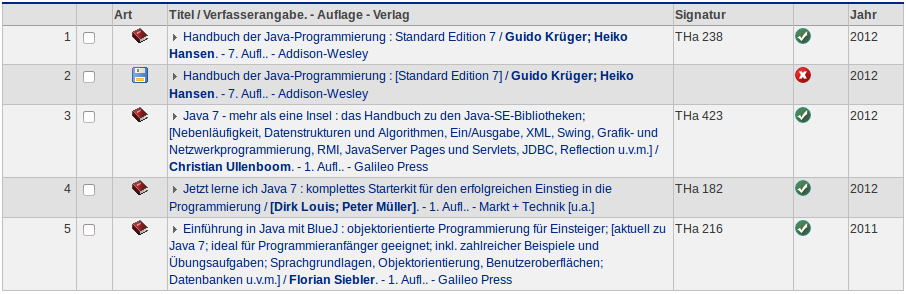
\includegraphics[width=\textwidth]{images/dhbw-lib-search-results.png}
\end{center}

Wir haben alle gelisteten Bücher zu Java 7 vor Ort in der Bibliothek gesichtet. Von den gelisteten Exemplaren ging nur ein Werk\cite{javainsel2} direkt auf die Neuerungen in Java 7 ein. Die anderen Fachbücher stellen eine allgemeine Beschreibungen der Java SE Bibliotheken dar denen lediglich Java in Version 7 zu Grunde liegt\cite{dhLibHandbuchJava} oder Sie richten sich gezielt nur an Javaanfänger\cite{dhLibJetztJavaLernen}\cite{dhLibBlueJStart}, wodurch sie für eine weitere Betrachtung im aktuellen Kontext nicht interessant sind.\\

Das Buch \glqq Java 7 - Mehr als eine Insel\grqq\cite{javainsel2} ~beschreibt in einem eigenen Kapitel die Neuerungen in Java 7. Der Autor, Christian Ullenboom, ist uns bereits durch seine frühere Veröffentlichung \glqq Java ist auch eine Insel\grqq\cite{javainsel1} ~bekannt gewesen, die mittlerweile als Referenzwerk für die Java SE Bibliotheken gehandelt wird. Die aktuelle Ausgabe dieses Buchs basiert ebenfalls auf Java 7 und kann im \glqq Stand der Technik\grqq ~Dokument verwendet werden.

\subsection{Offizielle Oracle-Ressourcen}\label{oracle}
Oracle stellt die Sprachänderungen an Java 7 unter anderem durch die Release
Notes\footnote{\url{http://www.oracle.com/technetwork/java/javase/jdk7-relnotes-418459.html}} mit dem Titel 
\glqq Java SE 7 Features and Enhancements\grqq\cite{oracleJavaRel}~vor. Darüber hinaus sind alle API-Funktionen in den 
Java-Docs\footnote{\url{http://docs.oracle.com/javase/7/docs/api/}}\cite{javadocs} dokumentiert.\\

Auch das Zertifizierungsprogramm der Oracle University\footnote{\url{education.oracle.com}} wurde auf die Sprachänderungen in Java 7 angepasst.
Die neuen Prüfungen 1Z0-803\footnote{\url{http://education.oracle.com/pls/web_prod-plq-dad/db_pages.getpage?page_id=5001&get_params=p_exam_id:1Z0-803}}, 
1Z0-804\footnote{\url{http://education.oracle.com/pls/web_prod-plq-dad/db_pages.getpage?page_id=5001&get_params=p_exam_id:1Z0-804}} und 
1Z0-805\footnote{\url{http://education.oracle.com/pls/web_prod-plq-dad/db_pages.getpage?page_id=5001&get_params=p_exam_id:1Z0-805}} 
erlauben die Zertifizierung zu Oracle Cetified Professional Java Programmer bzw. Associate.
Durch die neuen Zertifizierungen wird auch Lehrmaterial\footnote{\url{http://education.oracle.com/pls/web_prod-plq-dad/db_pages.getpage?page_id=640}}, 
bezogen auf die Sprachänderungen, bereit gestellt.\\

Bereits zu Java 6 erstellte, damals noch Sun, ein Lehrbuch\cite{scjp6} zur Zertifizierung. Die selben Autoren haben eine aktualisierte 
Version des Werks\cite{scjp7} für den 21.06.2013 angekündigt. Bisher ist bereits das Buch 
\glqq Oracle Certified Professional Java SE 7 Programmer Exams 1Z0-804 and 1Z0-805\grqq\cite{apressjava}~zur Vorbereitung erschienen.

\subsection{DPMA - Deutsches Patent- und Markenamt}

Wir haben die Einsteigersuche\footnote{http://depatisnet.dpma.de/DepatisNet/depatisnet?action=einsteiger} des DPMA verwendet um Patente mit Bezug zum Thema Java 7 zu finden. Eine Suche im Titel ergab hierbei für \glqq Java 7\grqq ~keinen Treffer und für \glqq Java \grqq ~2476 Treffer. In der Volltextsuche wurden für \glqq Java 7\grqq ~3521 Ergebnisse gefunden.\\

Um aktuelle Neuerungen zu finden wurde zusätzlich die Sortierung nach Veröffentlichungsdatum genutzt. Bei unserer Recherche war es in der Menge der Ergebnisse nicht möglich auch nur einen Eintrag aufzufinden, der sich auf Neuerungen in der Sprache bezieht. Alle betrachteten Einträge verwenden lediglich Java. Dar Java SE 7 an sich als Open Source verfügbar ist, ist es generell unwahrscheinlich das Patente auf offizielle Sprachänderungen an Java bestehen.\\

\subsection{ACM - Association for Computing Machinery}
Unter verwendung des Suchbegriff \glqq New Features in Java 7 \grqq ~wurden 45637 Treffer erzielt.
Weitere Suchbegriffe ergaben noch deutlich mehr Treffer.\\

Einige der aufgefundenen Artikel lassen einen Interessanten Inhalt, auch im Bezug auf das Thema dieser Arbeit, vermuten. Leider sind die gefunden Arbeiten in der Regel nur gegen Entgeld erhältlich, wodurch wir für weitere Betrachtungen andere Quellen bevorzugt haben.\\

Der vielversprechendste Treffer ist der Artikel \glqq An introduction to Java development kit 7 \grqq\cite{acmJava7} ~von Daryl Mayer, Nikola Grecevski und Vijay Sundaresan.

\subsection{Search Data Backup}
Eine Suche nach \glqq Java 7 Features\grqq\footnote{http://searchdatabackup.techtarget.com/search/query?q=Java+7+features} ~lieferte sehr viele Ergebnisse mit direktem Bezug zu den aktuellen Sprachänderungen. Aus der vielzahl der guten Ergebnisse musste selektiv ausgewählt werden. Wir haben die jenigen Artikel gewählt, die gezielt neue Features aus Java SE 7 vorstellen. So verblieben sechs Artikel in der Auswahl.\\

Ein Artikel\cite{sbJ7ImproveSec} betrachten den Einfluss neuer Features auf die Sicherheit von Java, ein Artikel\cite{sbJ7literals} beschreibt Änderungen an Literalen, vier Artikel stellen das Automated Resource Management\cite{sbJ7resources}\cite{sbJ7coin} neue Kontrollstrukturen\cite{sbJ7switch} und Supressed Exceptions\cite{sbJ7exeptions} vor.

\subsection{IEEE xplore}
Bei der IEEE xplore Digital Library steht eine unentgeltliche Titelsuche\footnote{http://ieeexplore.ieee.org/Xplore/guesthome.jsp} zur Verfügung. Eine Volltextsuche ist nur mit IEEE Mitgliedschaft\footnote{http://www.ieee.org/services/innovate/index2.html} möglich.\\

Die Suche nach \glqq Java\grqq ~ergab über 16.000 Treffer. Unter den 100 Treffern mit der größten Relevanz fanden sich keine nutzbaren Dokumente. Suchen nach \glqq Java 7\grqq ~und \glqq Java SE 7\grqq ~ergaben keine Ergebnisse.

\subsection{FIZ Technik / WFi Frankfurt}
Die Suchfunktion\footnote{http://www.fiz-technik.de/tecfinder/faces/facelets/search/search.jsp} zeigte sich uns äußerst schlecht bedienbar. Nich alle Browser werden durch die Seite unterstützt. Die bereits bei den vorherigen Recherchen genutzten Schlagworte ergaben zwar einige Resultate mit entferntem Bezug zum Thema, diese waren jedoch von schlechterer Qualität als bereits bekannte Dokumente. Von einer detaillierten Betrachtung haben wir daher abgesehen.
Für den Zugriff auf die Dokumente ist eine Registrierung\footnote{http://www.fiz-technik.de/tecfinder/faces/facelets/registration/registration.jsp} erforderlich.

\subsection{Milibib / Oldenbourg Akademie Link}
Eine Suche nach \glqq Java\grqq ~ergab 57 Titel\footnote{https://milibib.missing-link.de/}. Wir haben alle Titel gesichtet. Es bafanden sich vorwiegend Grundlagenbücher und allgemeine Werke zu Java darunter. Gezielt auf aktuelle Änderungen bezog sich keines der Bücher.\\

Für uns interssant ist das Werk \glqq Java 6 Core Techniken - Essentielle Techniken für Java-Apps\grqq\cite{java6core} ~von Friedrich Esser. Das Buch kann aus dem DHBW-Netz über Oldenbourg Akademie Link als E-Book\footnote{http://www.oldenbourg-link.com/isbn/9783486584110} bezogen werden. Das Kapitel \glqq Java 6 Basics\grqq\cite{java6core} ~sellt die Sprachänderungen von Java SE Version 5 zu Version 6 vor.

\subsection{Google}
Wie erwartet, bringt die Suche bei Google riese Treffermengen. So lieferte eine Suche nach \glqq Java 7 Änderungen\grqq~
1.440.000 Treffer, eine englische Suche nach \glqq Java 7 new features\grqq~gar 82.300.000 Ergebnisse. Da die Relevanz bei
Google sehr gut eingeschätzt wird, waren unter den ersten Suchergebnissen bei beiden Suchen sehr vielversprechende Artikel
und Bücher.\\

Eine gute Betrachtung aller kleinen Änderungen sowie den neuen Performance-Verbesserungen bietet der Artikel
\glqq Was ist neu in Java 7\grqq\cite{heiseWasistNeu}~auf Heise Developer.
Auch von Interesse ist der Artikel \glqq Java 7 Features\grqq\cite{blogJava7Features}~von Simon Koelsch, welcher sich nicht nur
den Änderungen an der Sprache sondern zusätzlich den Erweiterungen an der Virtuellen Maschine widmet.
Zusätzlich findet Google den Wikipedia-Artikel zu den verschiendenen Java-Versionen, worauf genauer in Kapitel TODO eingegangen wird.
Des Weiteren findet man bei Google das Buch \glqq Java 7 - Mehr als eine Insel\grqq\cite{javainsel2}, welches wir bereits in der
DHBW-Bibliothek gefunden hatten, sowie die Verlinkung zur Oracle Java 7 Homepage, die wir aber als eigene Quelle bereits
identifiziert hatten (siehe Kapitel TODO).

\subsection{Wikipedia}
Die Suche auf Wikipedia, unterstützt durch Google mit dem Suchbegriff \glqq java 7 wikipedia\grqq (83.100.000 Ergebnisse) ergab
fünf Artikel. Drei davon (\cite{wikiJavaSoftwarePlatform}, \cite{wikiJavaProgrammiersprache}, \cite{wikiJavaStandardEdition})
sind Artikel generell zu Java, ohne speziell auf Java 7 einzugehen. In den Artikeln \glqq Java-Technologie\grqq\cite{wikiJavaTechnologie}
~sowie \glqq Java version history\grqq\cite{wikiJavaVersionHistory}~wird zwar der Changelog von Java 7 aufgeführt, aber nicht
weiter beschrieben. Damit sind diese Quellen für uns nahezu unbrauchbar. Lediglich ein Abgleich der Vollständigkeit mit anderen
Artikeln ist uns damit möglich.

\subsection{Elektronische Zeitschriftenbibliothek}
Die Suche in der EZB brachte keine Resultate, bei den Suchbegriffen \glqq Java 7\grqq~sowie \glqq Java features\grqq~kamen
jeweils keine Treffer heraus. Lediglich bei einer Suche ganz allgemein nach \glqq Java\grqq~gab es 13 Treffer. Von diesen waren
nur zwei frei zugänglich, die aber keinerlei Relevanz für uns haben. Den Artikel \glqq State of the Art in Java Program Analysis
(SOAP)\grqq~hätten wir gerne näher betrachtet, leider war dieser aber nicht zugänglich.

\subsection{SpringerLink}
Bei der Suche auf SpringerLink kamen bei \glqq Java 7\grqq~72.242 Treffer heraus. Das zweite Ergebnis, das Buch \glqq Pro Java 7
NIO.2\grqq\cite{proJava7}~von Anghel Leonard aus dem Jahre 2011 sieht sehr vielversprechend aus, weil das Inhaltsverzeichnis
\footnote{\url{http://link.springer.com/book/10.1007/978-1-4302-4012-9/page/1}} (sowie der Titel) zeigt, dass es um viele der neuen
I/O-Funktionen von Java 7 geht.
Die anderen Treffer innerhalb der ersten 100 waren für uns nicht relevant.\\

Eine Suche mit dem Begriff \glqq Java 7 new features\grqq brachte 41.783 Treffer, von denen gleich der erste, ein Vergleich zwischen
Java und Ada sehr interessant zu sein schien. Leider stellte sich aber heraus, dass das Buch 
(\glqq A Comparison of the Object-Oriented Features of Ada 2005 and Java\grqq\cite{adacomparison}) von 2008 ist 
und damit auf jeden Fall keine aktuellen Konzepte zwischen den beiden Sprachen verglichen werden.
Der Titel des Buches brachte uns auf die Suchabfrage \glqq Java 7 comparison\grqq, um etwaige aktuellere Vergleiche zwischen
Java und anderen Sprachen zu finden. Leider war bei den 29.802 Ergebnissen, bis auf das eben schon gefundene, keine Relevanten
dabei.

%\subsection{Books24x7}
%Books24x7 ist ein kostenpflichtiges Online-Angebot, wo man nicht nur suchen, sondern die Bücher auch direkt elektronisch lesen
%kann. Jeder IBM Mitarbeiter hat dort einen, durch IBM finanzierten, Account.\\
%
%Die Suche nach \glqq Java 7\grqq~brachte 2302 Ergebnisse. Dort waren gute Java-Bücher dabei, jedoch nur eines, welches sich direkt
%mit Neuerungen aus Java 7 beschäftigt und zwar das schon im SpringerLink gefundene \glqq Pro Java 7 NIO.2\grqq\cite{b247nio2}. Der
%riesige Vorteil daran, es hier zu finden, ist, dass wir es direkt online benutzen können. 

\subsection{Books 24x7}
Books 24x7\footnote{http://www.books24x7.com} bietet ein gigantisches Sortiment an Fachbüchern von beeindruckender Qualität und Aktualität. Literatur war aus dieser Ressource sehr gut auffindbar und leicht zu verwenden. Alle angebotenen Fachbücher sich komplett online verfügbar. Als IBM Mitarbeiter steht uns ein uneingeschränkter Zugriff auf alle Quellen zur Verfügung.\\

Neben der Suchfunktion erleichtert die gute manuelle Kategorisierung der Bücher das Auffinden erheblich. Zu Java finden sich insgesamt (manuell kategorisiert) 2302 Bücher. Einige davon beziehen sich auch direkt auf Neuerungen in Java 7.\\

Ein wichtiges Teilprojekt von Java 7 sind I/O-Verbesserungen durch NIO.2. Dies war uns bereits bekannt. Mit dem Buch \glqq Pro Java 7 NIO.2\grqq\cite{b247nio2} ~von Anghel Leonard liegt uns nun eine umfassende Referenz hierzu vor, die sich gezielt an fortgeschrittene Java Experten richtet.

\begin{center}
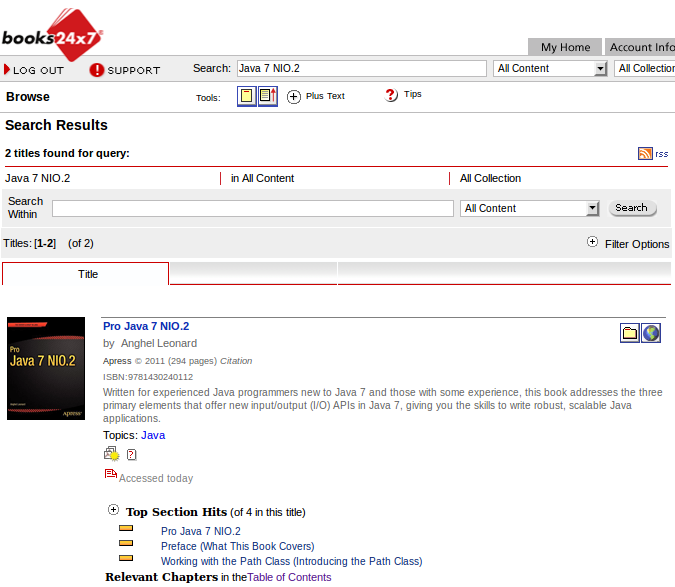
\includegraphics[width=10cm]{images/books247.png}
\end{center}

Auf Grund der gemachten Erfahrungen ist der Erwerb eines Zugangs zu dem Angebot\footnote{http://www.skillsoft.com/Books24x7/Product\_ Information/default.asp} für Informatiker auf jeden Fall empfehlenswert.

\subsection{Video2Brain}
Bei der Suche auf Video2Brain nach \glqq Java 7\grqq~(17 Treffer) stach direkt das Video-Tutorial \glqq Neu in Java 7\grqq\cite{v2bJava7}~
ins Auge, welches die wichtigstens Neuerungen von Java 7 kurz anhand von Code-Beispielen vorstellt.
Die anderen Ergebnisse waren nicht relevant.
%
%eof




